% Exemple de fichier LaTeX permettant de compiler des figures de circuits electriques en format "standalone"

% Example of a LaTeX file to compile electric circuits diagrams in standalone format
\documentclass[border = 5pt, tikz]{standalone} % Load packages needed for this TeX file:

\usepackage{tikz}
\usepackage{amsmath,amsthm,amssymb,amsfonts,relsize,mathrsfs}
\usepackage[siunitx]{circuitikz}
\usetikzlibrary{babel}

\begin{document} % Add your TeX code, e.g. a picture: \begin{tikzpicture}
\begin{tikzpicture}
\draw
(0,0) to[L, label=\mbox{$L$}] (0,4)
(0,4)to[C, label=\mbox{$C$}] (4,4)  to[american voltage source, label=\mbox{$V$}] (4,0) to[R, label=\mbox{$R_a+R_b$}] (0,0);
\end{tikzpicture}%
%
%%%%%%%%%%%%%%%%
\end{document}

% Exemple intégration de Circuit_compile.tex
% Voir la Figure~\ref{fig:Circuit} pour plus de détails. 

% \begin{figure}[htb]
% \centering
% 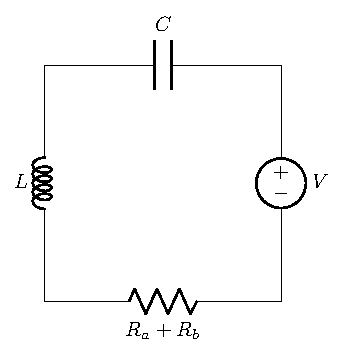
\includegraphics[width=2in]{Circuit_compile}
% \caption{Circuit}
% \label{fig:Circuit}
% \end{figure}